%%%%%%%%%%%%%%%%%%%%%%%%%%%%%%%%%%%%%%%%%%%%%%%%%%%%%%%%%%%%%%%%%%
%%%%%%%% ICML 2017 EXAMPLE LATEX SUBMISSION FILE %%%%%%%%%%%%%%%%%
%%%%%%%%%%%%%%%%%%%%%%%%%%%%%%%%%%%%%%%%%%%%%%%%%%%%%%%%%%%%%%%%%%

% Use the following line _only_ if you're still using LaTeX 2.09.
%\documentstyle[icml2017,epsf,natbib]{article}
% If you rely on Latex2e packages, like most moden people use this:
\documentclass{article}

% use Times
\usepackage{times}
% For figures
\usepackage{graphicx} % more modern
%\usepackage{epsfig} % less modern
\usepackage{subfigure} 

% For citations
\usepackage{natbib}

% For algorithms
\usepackage{algorithm}
\usepackage{algorithmic}

% As of 2011, we use the hyperref package to produce hyperlinks in the
% resulting PDF.  If this breaks your system, please commend out the
% following usepackage line and replace \usepackage{icml2017} with
% \usepackage[nohyperref]{icml2017} above.
\usepackage{hyperref}

% Packages hyperref and algorithmic misbehave sometimes.  We can fix
% this with the following command.
\newcommand{\theHalgorithm}{\arabic{algorithm}}

% Employ the following version of the ``usepackage'' statement for
% submitting the draft version of the paper for review.  This will set
% the note in the first column to ``Under review.  Do not distribute.''
\usepackage{icml2017} 

% Employ this version of the ``usepackage'' statement after the paper has
% been accepted, when creating the final version.  This will set the
% note in the first column to ``Proceedings of the...''
%\usepackage[accepted]{icml2017}
\usepackage{fullpage}
\usepackage{amsthm}
\usepackage{amssymb}
\newtheorem{theorem}{Theorem}[section]
\newtheorem{lemma}[theorem]{Lemma}
\newtheorem{fact}[theorem]{Fact}
\newtheorem{proposition}[theorem]{Proposition}
\newtheorem{observation}[theorem]{Observation}
\newtheorem{corollary}[theorem]{Corollary}
\newtheorem{remark}[theorem]{Remark}
\newtheorem{conjecture}[theorem]{Conjecture}
\newtheorem{definition}[theorem]{Definition}
\newtheorem{claim}[theorem]{Claim}
\newtheorem{assumption}{Assumption}

\usepackage{amsmath}
\usepackage{thmtools, thm-restate}
\usepackage{multirow}
\usepackage{tabularx}
\usepackage{colortbl}
\usepackage{color}
\usepackage[small]{caption}
%\usepackage[ruled,vlined]{algorithm2e}

\newcommand{\llabel}[1]{\label{#1}}
\newcommand{\heading}[1]{{\bf #1}}

\newcommand{\zo}{\{0,1\}}
\newcommand{\mzo}{\{-1,+1\}}
\newcommand{\F}{{\mathbb{F}}}
\newcommand{\N}{{\mathbb{N}}}
\newcommand{\Z}{{\mathbb{Z}}}
\newcommand{\R}{{\mathbb{R}}}
\newcommand{\C}{{\mathbb{C}}}
\newcommand{\eps}{\epsilon}
\newcommand{\beq}{\begin{eqnarray}}
\newcommand{\eeq}{\end{eqnarray}}
\newcommand{\tO}{\tilde{O}}
\newcommand{\bt}{\tilde{b}}
\newcommand{\vb}{{\bar b}}
\newcommand{\sign}{\text{sign}}
\newcommand{\T}{T}
\newcommand{\ip}[1]{\langle #1 \rangle}
\DeclareMathOperator{\Tr}{Tr}

\newcommand{\Vol}{\mathop\mathrm{Vol}\nolimits}
\newcommand{\Const}{\mathop\mathrm{Const}\nolimits}
\newcommand{\E}[2]{{\mathbb{E}_{#1}\left[#2\right]}}
\newcommand{\EE}[2]{{\mathbb{E}_{#1}{#2}}}
\newcommand{\EX}{{\mathbb E}}
\newcommand{\Sur}{\mathop\mathrm{Sur}\nolimits}
\newcommand{\polylog}{\mathop\mathrm{polylog}\nolimits}
\newcommand{\xor}{\oplus}
\newcommand{\conj}[1]{{\overline {#1}}} %% conjugate
\newcommand{\pd}[2]{\frac{\partial#1}{\partial#2}}

% The \icmltitle you define below is probably too long as a header.
% Therefore, a short form for the running title is supplied here:
\icmltitlerunning{Electron-Proton Dynamics in Deep Learning}

\begin{document} 

\twocolumn[
\icmltitle{Electron-Proton Dynamics in Deep Learning}

% It is OKAY to include author information, even for blind
% submissions: the style file will automatically remove it for you
% unless you've provided the [accepted] option to the icml2017
% package.

% list of affiliations. the first argument should be a (short)
% identifier you will use later to specify author affiliations
% Academic affiliations should list Department, University, City, Region, Country
% Industry affiliations should list Company, City, Region, Country

% you can specify symbols, otherwise they are numbered in order
% ideally, you should not use this facility. affiliations will be numbered
% in order of appearance and this is the preferred way.
\icmlsetsymbol{equal}{*}

\begin{icmlauthorlist}
\icmlauthor{Qiuyi Zhang}{berk,goo}
\icmlauthor{Rina Panigrahy}{goo}
\icmlauthor{Sushant Sachdeva}{goo}
\end{icmlauthorlist}

\icmlaffiliation{berk}{University of California Berkeley, Berkeley, California, USA}
\icmlaffiliation{goo}{Google Research, Mountain View, California, USA}

\icmlcorrespondingauthor{Qiuyi Zhang}{qiuyizhang@gmail.com}
\icmlcorrespondingauthor{Rina Panigrahy}{rinap@google.com}

% You may provide any keywords that you 
% find helpful for describing your paper; these are used to populate 
% the "keywords" metadata in the PDF but will not be shown in the document
\icmlkeywords{deep learning, theoretical machine learning, ICML}

\vskip 0.3in
]

% this must go after the closing bracket ] following \twocolumn[ ...

% This command actually creates the footnote in the first column
% listing the affiliations and the copyright notice.
% The command takes one argument, which is text to display at the start of the footnote.
% The \icmlEqualContribution command is standard text for equal contribution.
% Remove it (just {}) if you do not need this facility.

%\printAffiliationsAndNotice{}  % leave blank if no need to mention equal contribution
\printAffiliationsAndNotice{\icmlEqualContribution} % otherwise use the standard text.
%\footnotetext{hi}

\begin{abstract} 
We study the efficacy of learning neural networks with neural networks by the (stochastic) gradient descent method. While gradient descent enjoys empirical success in a variety of applications, there is a lack of theoretical guarantees that explains the practical utility of deep learning. We focus on two-layer neural networks with a linear activation on the output node. We show that under some mild assumptions and certain classes of activation functions, gradient descent does learn the parameters of the neural network and converges to the global minima. Using a node-wise gradient descent algorithm, we show that learning can be done in finite, sometimes $poly(d,1/\epsilon)$, time and sample complexity.
\end{abstract} 

\section{Introduction}

\subsection{Background}
Deep learning has been widely adopted to solve a variety of practical problems in artificial intelligence. From the perspective of learning theory, deep learning is the use of neural networks to approximate some target function $f: \R^n \to \R$, given training samples $(x_i,f(x_i))$ where $x_i$ is drawn according to some distribution $\mathcal{D}$. Standard algorithms are then used to perform empirical risk minimization (ERM) to find parameters that best fit our training data. Backpropagation, perhaps the most well-known algorithm in deep learning, applies stochastic gradient descent to squared loss to learn these suitable parameters. However, are these discovered parameters provably good or even optimal? 

The main difficulty in analysis is the non-convexity of the loss objectives that deep learning present. While convex optimization has been well studied and understood, there is relatively little known about provable guarantees in non-convex optimization. Recent work has shown that stochastic gradient methods will efficiently converge to a local minimizer and escape saddle points, under modest assumptions \cite{GeHJY15}. Therefore, it suffices to analyze the local minima of the loss landscape and show that no spurious local minima exist. This direction has led to positive results in matrix sensing \cite{ParkKCS16a}, matrix completion \cite{GeLM16}, dictionary learning \cite{SunQW15}, phase retrieval \cite{SunQW16}, and tensor decomposition \cite{GeHJY15}. A good overview of recent successes in the analysis of non-convex optimization in given in \cite{SunQW15a}.

A non-convex analysis of the deep learning objective has been largely elusive and more discouragingly, there has been hardness results for even simple networks. A neural network with one hidden unit and sigmoidal activation can admit exponentially many local minima \cite{Auer}. Backprogration has been proven to fail in a simple network due to the abundance of bad local minima \cite{brady1989back}. Training a 3-node neural network with one hidden layer is { NP}-complete \cite{BlumR88}.  But, these and many similar worst-case hardness results are based on worst case training data assumptions, which is arguably unrealistic. However, by using a result in \cite{klivans2006cryptographic} that learning a neural network with threshold activation functions is equivalent to learning intersection of halfspaces, several authors showed that under certain cryptographic assumptions, depth-two neural networks are not efficiently learnable with smooth activation functions \cite{LivniSS14} \cite{ZhangLWJ15}\cite{ZhangLJ15}. Related average-case hardness results for learning intersection of halfspaces are further expounded in \cite{daniely2014average}.

Due to the difficulty of analysis, many have turned to improper learning and the study of non-gradient descent methods to train neural networks. Janzamin et. al use tensor decomposition methods to learn the shallow neural network weights, provided access to the score function of the training data distribution \cite{JanzaminSA15}. Eigenvector and tensor methods are also used to train shallow neural networks with quadratic activation functions in \cite{LivniSS14}. Combinatorial methods that exploit layerwise correlations in sparse networks have also been analyzed provably in \cite{AroraBGM13}. Kernel methods, ridge regression, and even boosting were explored for regularized neural networks with smooth activation functions in \cite{shalev2011learning}\cite{ZhangLWJ15}\cite{ZhangLJ15}. Non-smooth activation functions, such as the ReLU, can be approximated by polynomials and are also amenable to kernel methods\cite{GoelKKT16}. These methods require assumptions that lessen the relevance of these algorithms to practice and more importantly, come short of explaining the widespread success of simple gradient descent.

Therefore, we will only focus on gradient-based methods in the proper learning framework and hope to find a theoretical justification of the good convergence properties. Thus far, most convergence proofs of applying gradient-based methods to neural networks can be obtained only under stringent assumptions. If the activation functions are linear or if certain independence assumptions are made, Kawaguchi shows that the only local minima are the global minima \cite{Kawaguchi16a}. Under other unrealistic assumptions, some authors have shown that the loss landscape admit well-behaving local minima that occur usually when the overall error is small \cite{ChoromanskaHMAL14},\cite{DauphinPGCGB14}. When only training error is considered, some authors have shown that a global minima can be achieved if the neural network contains sufficiently many hidden nodes, but doing so would overfit and lead to bad generalization error \cite{SoudryC16}. Our research is largely inspired by \cite{valiant2014learning}, in which the authors show that when the target functions are polynomials, gradient descent on neural networks with one hidden layer is shown to converge to low error, given a large number of hidden nodes. Furthermore, when complex perturbations are allowed and polynomial activation functions are used, there is a lack of robust local minima. 

\subsection{Our Contribution}

In this work, we ask the question: Can we use neural networks to learn neural networks with gradient descent methods? That is, if the function to be learnt is a neural network, and we try to learn it with a network of the same shape and randomly initialized edge weights, then will the gradient descent converge to the right function? Our experimental simulations show that for different widths and heights functions represented by neural networks with random edge weights can be learnt by stochastic gradient descent (see section~\ref{experiments}).

Next, we provide a theoretical justification with simplifying assumptions: specifically we will focus on learning depth two networks with a linear activation on the output node given by the form $f(x) = \sum_{i=1}^k b_i\sigma(x,w_i)$. Under some assumptions, we will show that gradient descent can learn the underlying weight parameters of the target network for certain activation functions. Specifically, we show convergence of the weight parameters of the trained network to those of the target network. The algorithm will try to learn a guess $\widehat{f}(x_j) = \sum_{i=1}^k a_i \sigma(x_j,\theta_i)$ for $f$ and then running gradient descent over the parameters $a_i, \theta_i$ will move them to $b_i, w_i$. 

\subsubsection{Gradient descent can be viewed as electron proton dynamics}
Our main observation is that the gradient descent dynamics of learning such to layer networks is equivalent to the dynamics of a set of proton-electron charges under a certain electrical attraction force function. Assume for now that the coefficients $b_i$ and $a_i$ are $1$. Thus we are only gradienting over $\theta_i$ to minimize the squared $l_2$ norm of the error function $f-\widehat{f}$ where $\widehat{f}(x_j) = \sum_{i=1}^k  \sigma(x_j,\theta_i)$.

\begin{theorem}(informal statement of Theorem~\ref{EPDyn})
The gradient descent process for learning $f$ is equivalent to the motion of k electrons in the presence of k fixed protons where the force between any pair of charges is given by a potential function that depends on $\sigma$.
\end{theorem}

The charges reside in $R^d$. The protons are fixed at locations $w_1,..,w_k$. The electrons are at positions $\theta_1,..,\theta_k$ and can move: the total force on each charge is the sum of the pairwise forces, in each infinitesimal time step $dt$ an electron moves by a distance proportional to the net force acting on it. Given this equivalence, the question is whether under this dynamic the electrons will eventually match up with the protons; this can be interpreted as $\theta_i$'s matching up with the $w_i$'s which means the function $f$ is learnt. 

\subsubsection{Analyzing electron proton convergence for different $\Phi$ and $\sigma$}

Note that for the standard electric potential function given by $\Phi = 1/r$ where $r$ is the distance between the charges, it is known that the electrons must converge with the protons, by Earnshaw's Theorem. However, there is no activation function $\sigma$ corresponding to this $\Phi$. 

We derive some sufficient conditions that characterize potentials that arise from activation functions $\sigma$. The different $\sigma$ that we study, their corresponding potentials, and their convergence results are summarized in Table ~\ref{table1}. Common activations used in practice are the sign and polynomial activation, for which we have derived show some results of convergence. We also construct synthetic activation functions for which convergence of the charges can be proven, implying we can learn the function $f$ in $poly(d,1/\epsilon)$ iterations of gradient descent.



\begin{table}[tb]
\caption{Potentials and Convergence Results Summary}
\label{table1}
\noindent
\vskip 0.1in
\begin{center}
\begin{small}
\begin{sc}
\begin{tabular}{
  |p{\dimexpr.28\linewidth-2\tabcolsep-1.3333\arrayrulewidth}% column 1
  |p{\dimexpr.4\linewidth-2\tabcolsep-1.3333\arrayrulewidth}% column 2
  |p{\dimexpr.3\linewidth-2\tabcolsep-1.3333\arrayrulewidth}|% column 3
  }
   \hline 
        Name of Activation&  Potential  ($\Phi(\theta,w)$)    & GD Convergence? \\ \hline 
        Sign & $1 - \frac{2}{\pi}\cos^{-1}(\theta^Tw)$       & Yes (Thm \ref{SignConv}, \ref{SignConv2})\\ 
         Hermite   & $(\theta^Tw)^m$       & Yes, $poly(d,1/\epsilon)$ (Thm \ref{PolyConv}) \\        
        Exponential       & $e^{\theta^Tw-1}$       & Yes, $e^{poly(d)}$ (Thm \ref{GaussStrict}) \\ 
        Synthetic  & Complicated  & Yes, $poly(d,1/\epsilon)$ (Thm \ref{eigConv})\\
        Gaussian  &  $e^{-\|\theta-w\|_2^2/2}$       & Yes, $e^{O(d)}$ (Thm \ref{GaussStrict}) \\
        Bessel    &  $e^{-\|\theta-w\|_1}$        & Yes for $d=1$ (Thm \ref{eigConvAS}) \\   
        \hline
\end{tabular}
\end{sc}
\end{small}
\end{center}
\vskip -0.1in
\end{table} 


Our main tool for analysis is to derive second-order information about our dynamics by using the Laplacian of the Hessian (or a submatrix of the Hessian) of our loss function. Together with some generalization error bounds and discrete optimization results, we can finally translate these convergence results into finite time convergence rates. We remark that our algorithms learn and return a neural network with the same architecture and number of hidden nodes as the target network. This is a big contrast to the improper learning setting of many proposed algorithms. 

We acknowledge that there is still a large gap between our developed theory and practice. However, our work can offer theoretical explanations and guidelines for the design of better activation functions or gradient-based training algorithms. For example, better accuracy and training speed were reported when using the newly discovered exponential linear unit (ELU) activation function in \cite{ClevertUH15} \cite{ShahKSS16}. We hope for more theory-backed answers to these and many other questions in deep learning.

In section 2, we introduce our framework and assumptions, and derive and derive the equivalence between gradient descent and electron-proton dynamics under a suitable potential. In section 3, we give an overview of our main results and techniques for showing convergence of gradient descent to learn the hidden parameters for depth-2 neural networks with specified activation functions, including some common activation functions, such as the sign and the polynomial. These convergence results are proven under ideal assumptions to simply illustrate our ideas. In section 4, we address the steps necessary to prove finite convergence guarantees using a node-wise gradient descent algorithm, dealing with errors introduced from approximation and discretization. In section 5, experimental results confirm that depth-2 neural networks can be learned by gradient descent with common activation functions but seem to discredit that claim for higher depth networks.  


\section{Deep Learning, Potentials, and Electron-Proton Dynamics}

\subsection{Preliminaries}

The target concept class $\mathcal{C}_{\sigma,k}$ of our learning procedure is the output of a two-layer neural network with linear output activation and has the form $f(x) = \sum_{i=1}^k b_i\sigma(x,w_i)$, where the sum is over $k$ hidden units scaled by output weights $b_i \in \R$ and $\sigma(x,w):\R^d \times \R^d\to \R$ is the activation function that takes in a hidden weight vector $w \in \R^d$ and the input vector $x \in \R^d$. Exponentially sized networks are too big to represent meaningful output functions so we work in the regime where $k = O(poly(d))$. For some distribution $\mathcal{D}$, we can given $n$ pairs of training data $(x_i, f(x_i))$, where $x_i$ are drawn i.i.d. from $\mathcal{D}$. Our hypothesis class is the same as the concept class and our loss function is the squared loss. In particular, if the true target function $f$ have truth parameters $b_i, w_i$, $i = 1,...,k$, and our current guess $\widehat{f}$ has parameters $a_i, \theta_i$, $i=1...,k$, then we use the standard $l_2$ error.
\begin{equation}\label{errEmp}
\widehat{L}(a,\theta)  = \frac{1}{n}\sum_{j=1}^n \left(\sum_{i=1}^k b_i\sigma(x_j,w_i) - \sum_{i=1}^k a_i \sigma(x_j,\theta_i)\right)^2
\end{equation}
Instead of analyzing the optimization of \eqref{errEmp} and then arguing about generalization error, since the Rademacher complexity of $C_{\sigma, k}$ under reasonable assumptions is  $poly(k, d)/\sqrt{n}$, we would rather work with the true loss directly: $L(a,\theta) = {E}[\widehat{L}]$. This avoids overfitting concerns and forcing our algorithm to return a size $k$ network will also guarantee that we do not artificially enlarge our learned network. To further simplify $L$, let us parametrize $a$ with $-a$ and expand.
\begin{equation*}
L(a,\theta)  = \underset{X\sim D}{E}\left[ \left(  \sum_{i=1}^k a_i \sigma(X,\theta_i) + \sum_{i=1}^k b_i\sigma(X,w_i)\right)^2\right]
\end{equation*}
\begin{equation*}
= \sum_{ij} a_i a_j E[\sigma(X,\theta_i)\sigma(X,\theta_j)]  + 2 a_ib_j E[\sigma(X,\theta_i)\sigma(X,w_j)] 
\end{equation*}
Note that we have dropped the constant terms and if we let $\Phi(\theta, w) = E_{X\sim D}[ \sigma(X,\theta) \sigma(X,w)]$ be the {\bf potential function} {\it corresponding to the activation function} $\sigma$, then we finally have our loss function.
\begin{equation}\label{errLoss}
\begin{split}
L(a,\theta) &= \sum_{i=1}^k a_i^2 \Phi(\theta_i,\theta_i) + 2\sum_{i=1}^k\sum_{i < j} a_i a_j \Phi(\theta_i,\theta_j) \\
&+ 2\sum_{i=1}^k\sum_{j=1}^k a_ib_j \Phi(\theta_i,w_j)
\end{split}
\end{equation}
We will adopt standard manifold optimization notation in this paper. Let $\mathcal{M}$ denote our manifold in $\R^d$, usually either $\mathcal{M}= \R^d$ or $\mathcal{M} =  S^{d-1}$. All gradients and other operators are implicitly done with respect to $\mathcal{M}$.  If $f$ is multivariate with variable $x_i$, let $\nabla_{x_i}f, \Delta_{x_i}f$ to be the gradient and Laplacian, respectively, of $f_{x_i}$ on $\mathcal{M}$ with respect to $x_i$. Lastly, we say $x$ is a critical point of $f$ if $\nabla f$ does not exist or $\nabla f = 0$.

A gradient-based method is an algorithm that calls Algorithm \ref{GD} in all the optimization procedures to minimize the empirical loss. Given $\mathcal{D}$, the training data, and the activation function $\sigma$, we attempt to show that with high probability over some random choices of $b_i, w_i$, there exists a gradient-based algorithm that optimizes $\widehat{L}$ on $\mathcal{M}$ and finds $\widehat{f} \in \mathcal{C}_{\sigma, k}$ with probability $1-\delta$ such that $L(a,\theta) <\epsilon$, in time $poly(d,k,1/\delta,1/\epsilon)$ or some other meaningful bound.

\begin{algorithm}[hb]
 \caption{$x = GradientDescent(L,x_0, T,\alpha$)}
   \label{GD}
\begin{algorithmic}
   \STATE {\bfseries Input:} $L: \mathcal{M} \to \R$; $x_0 \in \mathcal{M}$; $T\in \N$; $\alpha\in \R$
   \STATE Initialize $x = x_0$
   \FOR{$i=1$ {\bfseries to} $T$}
   \STATE $x = x - \alpha\nabla L(x)$
   \STATE $x = \Pi_\mathcal{M} x$
   \ENDFOR
\end{algorithmic}
\end{algorithm}

\subsection{Electron-Proton Dynamics}

Observe that the first term in \eqref{errLoss} is often a constant in the variable $\theta$. Therefore, when $a_i$ are fixed, we will work with the simplified loss:
\begin{equation}\label{errSimp}
L(a,\theta) =  2\sum_{i=1}^k\sum_{i < j} a_ia_j\Phi(\theta_i,\theta_j) + 2\sum_{i=1}^k\sum_{j=1}^ka_ib_j \Phi(\theta_i,w_j)
\end{equation}
By interpreting the pairwise potentials as electrostatic attraction potentials, we notice that our dynamics is similar to electron-proton type dynamics under some potential $\Phi$, where $w_i$ are fixed point charges in $\R^d$ and $\theta_i$ are moving point charges in $\R^d$ that are trying to find $w_i$. 

\begin{definition}\label{EPDef}
Given a potential $\Phi : \mathcal{M} \times \mathcal{M} \to \R$ and particle locations $\theta_1,...,\theta_k \in \mathcal{M}$ along with their respective charges $a_1,...,a_k \in \R$. We define {\bf Electron-Proton Dynamics} under $\Phi$ to be the solution $(\theta_1(t),...,\theta_k(t))$ to the following system of differential equations: For each pair $(\theta_i,\theta_j)$, there is a force from $\theta_j$ exerted on $\theta_i$ that is given by ${\bf F}_{i}(\theta_j) = a_ia_j\nabla_{\theta_i} \Phi(\theta_i,\theta_j)$ and
\[-\frac{d\theta_i}{dt} =  \sum_{ j \neq i} {\bf F}_{i}(\theta_j)\]
for $i \in [k]$, with $\theta_i(0) = \theta_i$. If some subset $S \subseteq [k]$ of particles are fixed, then for $i\in S$, we have instead $\theta_i(t) = \theta_i$ for $t \geq 0$.

\end{definition}


\begin{theorem}\label{EPDyn}
Assume $\Phi(\theta, \theta)$ is constant. Running continuous gradient descent on \eqref{errLoss} with respect to $\theta$, initialized at $(\theta_1,...,\theta_k)$ produces the same dynamics as Electron-Proton Dynamics under $\Phi$ with fixed particles at $w_1,...,w_k$ with respective charges $b_1,..,b_k$ and moving particles at $\theta_1,...,\theta_k$ with respective charges $a_1,...,a_k$.
\end{theorem}

\begin{proof}
The initial values are the same. Notice that continuous gradient descent on $\frac{1}{2}L(a,\theta)$ with respect to $\theta$ produces dynamics given by $\frac{d\theta_i(t)}{dt} = -\nabla_{\theta_i}L(a,\theta)$. Therefore,
\[\frac{d\theta_i(t)}{dt} = -\sum_{j \neq i} a_i a_j \nabla_{\theta_i}\Phi(\theta_i,\theta_j) - \sum_{j=1}^k a_ib_j\nabla_{\theta_i} \Phi(\theta_i,w_j)\]
And gradient descent does not move $w_i$. By definition, the dynamics corresponds to Electron-Proton Dynamics as claimed.
\end{proof}

\subsection{Activation-Potential Correspondence}

We restrict our attention to potential functions with some natural symmetry, so they are either translationally or rotationally invariant. In particular, we may write $\Phi= h(x-w)$ for some function $h(x)$  in the first case and in the second case, $\Phi = h(x^Tw)$. We focus mainly on rotationally invariant potentials, as they correspond to classical neural networks, and we further make the normalizing assumption that $\theta, w \in S^{d-1}$. We remark that these assumptions allows us to conclude that $\Phi(\theta,\theta)$ {\it is always a positive constant and we also normalize $\Phi(\theta,\theta) = 1$ for the rest of the paper.}

We make another distributional assumption that our distribution $\mathcal{D} = \mathcal{N}(0, {\bf I_{d\times d}})$ is fixed as the standard Gaussian in $\R^d$. This assumption is not critical and a simpler distribution might be even better when considering sample complexity. However, if we allow arbitrary distributions, then they can be adversarially constructed and hardness results in PAC-learning halfspaces would apply \cite{klivans2006cryptographic}. 

\begin{definition}
Let $\mathcal{M} \subseteq \R^d$. We call $\Phi: \mathcal{M} \times \mathcal{M} \to \R$ a {\bf realizable} potential function if there exists a corresponding activation function $\sigma:\R^d \times \R^d \to \R$ bounded almost everywhere such that for all $\theta, w \in \mathcal{M}$,
\[\Phi(\theta,w) = E_{X \sim \mathcal{D}}[\sigma(X,\theta)\sigma(X,w)]\]
\end{definition}

We briefly state some results about characterizations of realizable potentials for translationally and rotationally invariant potentials. Full proofs and calculations of activation-potential correspondences, such as those claimed in Table \ref{table1}, are in the supplementary material.
 
\begin{restatable}{theorem}{tranReal}
\label{thm:tranReal}
Let $\mathcal{M} = \R^d$ and $\Phi(\theta,w) = f(\theta - w)$. Then, $\Phi$ is realizable if $\mathfrak{F}(f)(\omega) \geq 0$ and $\mathfrak{F}^{-1}(\sqrt{\mathfrak{F}(f)})$ is bounded almost everywhere, where $\mathfrak{F}$ is the standard fourier transform in $\R^d$
\end{restatable}




\begin{restatable}{theorem}{rotReal}
\label{thm:rotReal}
Let $\mathcal{M} = S^{d-1}$ and $\Phi(\theta,w) = f(\theta^Tw)$. Then, $\Phi$ is realizable if $f$ has non-negative Taylor coefficients, $c_i \geq 0$ , and 
\[h(x) = \sum_{i=1}^\infty \sqrt{c_i} h_i(x)\]
converges almost everywhere, where $h_i(x)$ is the i-th Hermite polynomial.
\end{restatable}

We remark these theorems are strong characterizations of realizable potentials, as converses to these theorems can be derived under more technical assumptions that we will avoid here. Such results usually hinge on the fact that $\Phi$ is a positive semi-definite kernel; for example, Bochner's theorem allows us to directly conclude that $\mathfrak{F}(f) \geq 0$. For the more interested reader, a good introduction is \cite{Fasshauer_positivedefinite}. 


\section{Main Results} 

\subsection{Earnshaw's Theorem}

When running gradient descent on non-convex loss functions, we often can and do get stuck at a local minima. In this section, we use second-order information to deduce the non-existence of such local minima. Earnshaw's theorem in electrodynamics shows that there is no stable local minima for electron-proton dynamics. This hinges on the property that the electric potential is harmonic. 

\begin{definition}
$\Phi(\theta,w)$ is a {\bf harmonic} potential on $\Omega$ if $\Delta_\theta \Phi(\theta,w) = 0$ for all $\theta \in \Omega$, except possibly at $\theta = w$.
\end{definition}

\begin{definition}
Let $\Omega \subseteq \R^d$ and consider a function $f:\Omega \to \R$. A critical point $x^* \in \Omega$ is a {\bf local minimum} if $\lambda_{min}(\nabla^2 f(x^*)) \geq 0$ and it is a {\bf strict local minimum}  if  $\lambda_{min}(\nabla^2 f(x^*)) > 0$.
\end{definition}

\begin{theorem}\label{Earnshaw} \cite{arnold1985mathematical}[Earnshaw]
Let $\mathcal{M}\subseteq \R^d$ and let $\Phi$ be harmonic. Then, $(a,\theta)$ is not a strict local minima of \eqref{errSimp} if there exists $i$ such that $\theta_i \neq w_j$ for all $j$ and $\theta_i \neq \theta_j$ for all $j\neq i$.
\end{theorem}

\begin{proof}
Consider $\theta_i$ such that $\theta_i \neq w_j, \theta_j$. Thus, our loss function $L$ in \eqref{errSimp} is twice differentiable with respect to $\theta_i$. If $(a,\theta)$ is a strict local minima, we must have
\[\nabla_{\theta_1} L = 0, \text{ and }  \Tr(\nabla^2_{\theta_i}L) > 0\]
But since $\Phi$ is harmonic,
\[ \Tr(\nabla^2_{\theta_i}L(q_1,...,q_n)) = \Delta_{\theta_i} L\]
\[ =  2\sum_{ j\neq i} a_ia_j \Delta_{\theta_i}\Phi(\theta_i,\theta_j) + 2\sum_{j=1}^ka_ib_j  \Delta_{\theta_i}\Phi(\theta_i,w_j) = 0\]
\end{proof}

\begin{corollary}
Let $\mathcal{M} = \R^d$, $\Phi(\theta,w) = \|\theta-w\|^{2-d}$, and $L$ be as in \eqref{errSimp}. If $\theta_i$ are all distinct and $(a,\theta)$ is a strict local minima, then $\theta$ has reached the global minima, i.e. $\theta_i = w_{\pi(i)}$ for some permutation $\pi$. 
\end{corollary}

Intuitively, the trace of the Hessian being 0 implies every differentiable critical point has a direction of negative curvative (unless the Hessian is the zero matrix altogether, in which case some complex analysis still finds a direction of negative change \cite{arnold1985mathematical}). Therefore, at convergence, we should expect $\theta_i = w_{\pi(i)}$ for some permutation $\pi$, as long as $\theta_i$ are all distinct. 

Such a result is desired but we run into two main problems. First, the singularity of the natural harmonic potentials at $0$ disqualifies them from being a realizable potential. Furthermore, harmonic potentials are not robust to approximation and statistical error as the convergence guarantees hinge on $\Delta_\theta\Phi$ being exactly 0. 

Second, the lack of strict local minima {\it does not} imply convergence to the global minima under gradient descent. Notice that harmonic potentials can admit local minima, as the Hessian matrix can be the zero matrix, and so gradient descent could converge to these local minima. However, if our loss function admits no local minima (other than the global minima), then we can guarantee that gradient descent with small stepsize converges to the global minima. 

\subsection{Alternative Notions of Harmonic Potentials}

\subsubsection{Strictly Subharmonic Potentials}

The first alternative to harmonic potentials is the natural consideration of strictly subharmonic potentials, which have a positive Laplacian value almost everywhere. 

\begin{definition}
$\Phi(\theta,w)$ is a {\bf strictly subharmonic} potential on $\Omega$ if $\Delta_\theta \Phi(\theta,w) > 0$ for all $\theta \in \Omega$, except at $\theta = w$.
\end{definition}


In this case, the sign of the output weights $a_i, b_i$ matter in determining the sign of the Laplacian of our loss function. Therefore, we need to make suitable assumptions in this framework.

\begin{assumption}
\label{outputFixed}
All output weights $b_i = 1$ and therefore the output weights  $a_i = - b_i = -1$ are fixed throughout the learning algorithm. 
\end{assumption}

Assumption \ref{outputFixed} is necessary to eliminate the possibility of spurious local minima in our framework, as counterexamples can be constructed in their absence. Now, we are working with the following loss function:
\begin{equation}\label{errFixed}
L(\theta) =  2\sum_{i=1}^k\sum_{i < j} \Phi(\theta_i,\theta_j) - 2\sum_{i=1}^k\sum_{j=1}^k\Phi(\theta_i,w_j)
\end{equation}
\begin{theorem}
Let $\Phi$ be strictly subharmonic on $\mathcal{M}$ and let Assumption \ref{outputFixed} hold. Let $L$ be as in \eqref{errFixed} and $x_0 \in \mathcal{M}$ randomly chosen. Then, all critical points of $L$ are not local minima, except at the global minima. 
\end{theorem}

\begin{proof}
To gain intuition, let $\Phi$ be translationally invariant and $\mathcal{M} = \R^d$. Let $\theta = (\theta_1,...,\theta_k)$ be a critical point. Assume, for sake of contradiction, that for all $i, j$, $\theta_i \neq w_j$. 

The main technical detail is to remove interaction terms between pairwise $\theta_i$ by considering a correlated movement, where each $\theta_i$ are moved along the same direction $v$. In this case, notice that our objective, as a function of $v$, is simply
\[L(v) =  2\sum_{i=1}^k\sum_{i < j} \Phi(\theta_i+v,\theta_j+v) - 2\sum_{i=1}^k\sum_{j=1}^k \Phi(\theta_i+v,w_j)\]

Note that the first term is constant as a function of $v$, by translation invariance. Therefore,
\[\nabla^2 L = -2\sum_{i=1}^k \sum_{j=1}^k \nabla^2\Phi(\theta_i, w_j)\]
By the subharmonic condition, $tr(\nabla^2L) = -2\sum_{i=1}^k\sum_{j=1}^k \Delta_{\theta_i}\Phi(\theta_i,w_j) < 0$. Therefore, we conclude that $\theta$ is not a local minima of $L$.

WLOG, let's say $\theta_1 = w_1$. Then, simply realize that we can write $L$ with $\theta_1,w_1$ terms cancelled out. We reduce to the case where we have $k-1$ variable charges and $k-1$ fixed charges, so by induction, we conclude that $\theta_i = w_{\pi(i)}$ for some permutation $\pi$. The above technique generalizes to $\Phi$ being rotationally invariant case by working in spherical coordinates and correlated translations are simply rotations. 
\end{proof}


Subharmonic potentials are also difficult to realize; however their convergence properties are more robust than harmonic potentials. In section 4, we prove convergence properties of approximations of strictly subharmonic potentials.


\subsubsection{$\lambda$-Harmonic Potentials (Laplacian Eigenfunctions)}

When we drop Assumption \ref{outputFixed} and allow the output weights to be variable and possibly negative, then our techniques above will not apply directly. However, notice that our loss function \eqref{errLoss} is quadratic in $a$, so convergence in the output weights is guaranteed. Let $a^*(\theta)$ denote the optimal set of output weights for a given $\theta$. Since $a^*$ is Lipschitz in $\theta$, it suffices to just reason about the convergence of the hidden weights $\theta_i$.

In order to relate our loss function with its Laplacian, we consider potentials that are non-negative eigenfunctions of the Laplacian operator. Since the zero eigenvalue case simply gives rise to harmonic potentials, we restrict our attention to positive eigenfunctions.

\begin{definition}
A potential $\Phi$ is {\bf$\lambda$-harmonic} on $\Omega$ if it is a positive eigenfunction of the Laplacian operator on $\Omega$ and there exists $\lambda > 0$ such that for every $\theta \in \Omega, \theta \neq w$,
\[\Delta_\theta \Phi(\theta, w) = \lambda \Phi(\theta,w) \]
\end{definition}

\begin{restatable}{lemma}{eigStrict}
\label{EigStrict}
Let $\Phi$ be $\lambda$-harmonic. For a point $(a,\theta)$, assume that $\theta_i \neq w_j$ for any $j$ and $\theta_i \neq \theta_j$ for some $j \neq i$. Then, if $a_i = a^*_i\neq 0$, then $(a,\theta)$ is not a local minima point of the \eqref{errLoss}.
\end{restatable}
\begin{proof}
Now, $a_i^*$ being optimal implies
\[0 = \pd{L}{a_i} = 2a_i \Phi(\theta_i,\theta_i) + 2\sum_{j\neq i} a_j \Phi(\theta_i,\theta_j) + 2\sum_{j=1}^k b_j \Phi(\theta_i,w_j)\]
Now, since $\theta_i$ is distinct from $w_j$ and other $\theta_j$, we can compute the Laplacian with respect to $\theta_i$ gives
\begin{align*}
\Delta_{\theta_i}L &= 2\sum_{j\neq i} a_i a_j \Delta_{\theta_i}\Phi(\theta_i,\theta_j) + 2\sum_{j=1}^k a_i b_j \Delta_{\theta_i}\Phi(\theta_i,w_j) \\
&= \lambda a_i\left(2\sum_{j\neq i} a_j \Phi(\theta_i,\theta_j) + 2\sum_{j=1}^k  b_j \Phi(\theta_i,w_j)\right) \\
&= -2\lambda a_i^2\Phi(\theta_i,\theta_i) = -2c \lambda a_i^2\\
\end{align*}
If $a_i^2 \neq 0$, then we conclude that the Laplacian is strictly negative, implying our claim.
\end{proof}

We note that there are realizable versions of these potentials; for example $\Phi(a,b) = e^{-\|a-b\|_1}$ in $\R^1$ can be realized. In Section 4, we show that approximations of these potentials are robust and retain good convergence behavior. 

\subsection{Realistic Potentials}

The analysis of convergence through Laplacian information do not directly extend to analyzing potentials that correspond to more widely-used activation functions in the deep learning community, such as sign, ReLU, or polynomial. However, for these more realistic potentials, we can still make some progress under further assumptions. 

Analyzing standard gradient descent on \eqref{errLoss} is complicated by pairwise interaction terms between $\theta_i, \theta_j$; our techniques in the previous section do not generalize well. Therefore, in this section, we only consider the convergence guarantee of gradient descent on the first node, $\theta_1$, to some $w_j$, while the other nodes are inactive (i.e. $a_2,...,a_k = 0$). In essence, we are working with the following simplified loss function.
\begin{equation}\label{errLossUnit}
L(a_1,\theta_1) =  a_1^2 \Phi(\theta_1,\theta_1)  + 2\sum_{j=1}^k a_1b_j \Phi(\theta_1,w_j)
\end{equation}
While a convergence result of \eqref{errLossUnit} is weaker, it motivates the introduction of a node-wise gradient descent algorithm, where instead of applying gradient descent on all $\theta_i$ simultaneously, we run gradient descent on $\theta_1,...,\theta_k$ sequentially. Under node-wise gradient descent, we can argue that each $\theta_i$ will be paired to some $w_j$ and then argue that such a matching is perfect. We will introduce and apply node-wise gradient descent to derive finite time bounds in Section 4.
\begin{theorem}
\label{PolyStrict}
Let $\mathcal{M} = S^{d-1}$. Let $w_1,...,w_k$ be orthonormal vectors in $\R^d$ and $\Phi$ is of the form $\Phi(\theta,w) = (\theta^Tw)^l$ for some fixed integer $l \geq 3$. Let $L$ be as in \eqref{errLossUnit}. Then, all critical points of $L$ are not local minima, except at the global minima. 
\end{theorem}
\begin{proof}
WLOG, we can consider $w_1,...,w_d$ to be the basis vectors $e_1,...,e_d$. Note that this is a manifold optimization problem, so our optimality conditions are given by introducing a Lagrange multiplier $\lambda$, as in \cite{GeHJY15}.
\[\pd{L}{a} = 2\sum_{i=1}^d ab_i (\theta_i)^l + 2a = 0\]
\[ (\nabla_\theta L)_i = 2ab_il(\theta_i)^{l-1}  -2\lambda \theta_i = 0 \]
where $\lambda$ is chosen that minimizes 
\[\lambda = \arg \min_\lambda \sum_i (ab_i l (\theta_i)^{l-1} - \lambda\theta_i)^2 = \sum ab_i l (\theta_i)^l \]
Therefore, either $\theta_i = 0$ or $b_i (\theta_i)^{l-2} = \lambda/(al)$. Note also that the manifold Hessian is a diagonal matrix with diagonal entry: 
\[(\nabla^2 L)_{ii} = 2a b_i l(l-1)(\theta_i)^{l-2} - 2 \lambda\]
Assume that there exists $\theta_i, \theta_j \neq 0$, then we claim that $\theta$ is not a local minima.  First, our optimality conditions imply $b_i(\theta_i)^{l-2} = b_j (\theta_j)^{l-2} = \lambda/(al)$. So,
\[(\nabla^2 L)_{ii} = (\nabla^2L)_{jj} = 2a b_i l(l-1)(\theta_i)^{l-2} - 2 \lambda\]
\[ = 2(l-2)\lambda = -2(l-2)la^2\]
Now, there must exist a vector $v \in S^{d-1}$ such that $v_k = 0$ for $k \neq i,j$ and $v^T\theta = 0$, so $v$ is in the tangent space at $\theta$. Finally, $v^T(\nabla^2 L) v  = -2(l-2)l a^2 < 0$, implying our claim when $a \neq 0$. Note that $a = 0$ occurs with probability 0 since our objective function is non-increasing throughout the gradient descent algorithm and is almost surely initialized to be negative with $a$ optimized upon initialization.
\end{proof}

Next, we consider the sign activation function. Under restrictions on the size of the input dimension or the number of hidden units, we can prove convergence results under the sign activation function. The sign activation function is problematic because it is not smooth and has a zero gradient almost everywhere. While statistical error bounds do not hold in the strict sense, we believe that these continuous convergence results could still shed light on sign-like functions, of which many are Lipschitz and enjoy generalization bounds. 

\begin{theorem}
\label{SignConv}
Let $\mathcal{M} = S^1$ and $k$ be the number of hidden nodes. Let $L$ be as in \eqref{errLossUnit} and $\sigma$ is the sign activation function. Then, almost surely over random choices of $b_1,...,b_k$, all critical points of $L$ are at $\pm w_j$.
\end{theorem}

\begin{proof}
In $S^1$, notice that the pairwise potential function is $\Phi(\theta,w) = 1 - 2\cos^{-1}(\theta^Tw)/\pi = 1 - 2\alpha/\pi$, where $\alpha$ is the angle between $\theta, w$. So, let us parameterize in polar coordinates, calling our true parameters as $\widetilde{w_1},...,\widetilde{w_k} \in [0,2\pi]$ and rewriting our loss as a function of $\widetilde{\theta} \in [0,2\pi]$. 

Since $\Phi$ is a linear function of the angle between $\theta, w_j$, each $w_j$ exerts a constant gradient on $\widetilde{\theta}$ towards $\widetilde{w_j}$, with discontinuities at $\widetilde{w_j},\pi+\widetilde{w_j}$. Almost surely over $b_1,..,b_k$, the gradient is non-zero almost everywhere, except at the discontinuities, which are at $\widetilde{w_j}, \pi+\widetilde{w_j}$ for some $j$. 
\end{proof}



\begin{corollary}
\label{SignConv2}
Let $\mathcal{M} = S^{d-1}$ and let there be $k$ hidden nodes with $k\leq 2$. Let $L$ be as in \eqref{errLossUnit} and $\sigma$ is the sign activation function. Then, almost surely over random choices of $b_1,...,b_k$, all critical points of $L$ are at $\pm w_j$.
\end{corollary}

\begin{proof}
Let $w_1,w_2$ be the two hidden weights. As shown in Theorem \ref{SignConv}, there is a constant force gradient
of $w_1, w_2$ on $\theta$. The set of points where the sum of the two forces can be 0 lies on the great circle passing though $w_1,w_2$. Therefore, it reduces to a problem in $S^1$, whose convergence is shown in Theorem \ref{SignConv}.
\end{proof}

We conjecture that for the sign potential function, convergence results can be derived when running gradient descent on all $\theta_i$ simultaneously. Because $\R^d$ is a simpler manifold to work with than $S^{d-1}$, we also conjecture that for the distance potential, convergence results hold. Note that the distance potential behaves like the sign function in polar coordinates as $\Phi(\theta, w)$ admits a constant norm gradient in the direction towards $w$. Therefore, convergence of the distance potential is implied by convergence of the sign potential. 

\begin{conjecture}
 Let $\mathcal{M} = S^{d-1}$ and let $k = poly(d)$ be the number of hidden nodes and let $L$ be as in \eqref{errLoss}. Let $\Phi$ be the potential corresponding to $\sigma(\theta,w) = sgn(\theta^Tw)$. Then, all critical points $(a,\theta)$ of $L$ with $a \neq 0$ are not local minima, except at the global minima. 
\end{conjecture}

\begin{conjecture}
 Let $\mathcal{M} = \R^d$ and let $k = poly(d)$ be the number of hidden nodes and let $L$ be as in \eqref{errLoss}. Let $\Phi$ be the distance potential $\Phi(\theta,w) = \|\theta - w\|$. Then, all critical points $(a,\theta)$ of $L$ with $a \neq 0$ are not local minima, except at the global minima.
\end{conjecture}


\section{Runtime Bounds with Stochastic Gradients}

The gradient descent convergence results in the previous sections lay the foundation for reasoning about the convergence of stochastic gradient descent (SGD) in standard backpropagation. To derive finite runtime bounds, we need to address three technical details: 1) realizable potentials are only approximately strict subharmonic or $\lambda$-harmonic, 2) the variance of the computed gradient due to generalization error is small and 3) SGD should escape local minima in a finite (hopefully polynomial) amount of time. In this section, we mainly address the first detail and state our finite convergence results for certain realizable potentials. 

The second and third detail are analyzed with standard techniques in optimization and statistics: the former requires generalization bounds for neural networks and the latter requires a lower bound on the negative curvature, which leads to the follow definition.

\begin{definition} Let $\Omega \subseteq \R^d$. A point $x^*$ is a {\bf $\epsilon$-strict} point of $f : \Omega \to \R$ if f is twice differentiable at $x^*$ and $\lambda_{min}(\nabla^2f(x^*)) < -\epsilon$
\end{definition}

Note that if a critical point is not a local minimum, then it is $0$-strict. It can be shown that SGD can avoid all points that are $\epsilon$-strict in $poly(1/\epsilon)$ iterations and will converge to a point in $\mathcal{M}_\epsilon$, where

\[\mathcal{M}_\epsilon = \left\{x\in \mathcal{M} \Big| \|\nabla L(x)\| \leq \epsilon \text{ and } \lambda_{min}(\nabla^2 L(x)) \geq -\epsilon\right\}\]

Intuitively, this means that SGD will converge to points with small gradient and small negative curvature. The full details are found in supplementary material. 

However, because of the introduced errors, we cannot simply analyze the convergence of SGD on all $\theta_i$ simultaneously since as before, the pairwise interaction terms between the $\theta_i$ present complications. To derive a tighter control on $(a,\theta)$, we run a greedy node-wise SGD algorithm to learn the hidden weights, i.e. we run a full SGD algorithm with respect to $(a_i,\theta_i)$ sequentially. The main idea is that after running SGD with respect to $\theta_1$, $\theta_1$ should be close to some $w_j$ for some $j$. Then, we can carefully induct and show that $\theta_2$ must be some other $w_k$ for $k\neq j$ and so on.

In addition, we remark that node-wise SGD allows us to learn the value of $k$, the number of hidden nodes in the target function. This may suggest that node-wise SGD serves as a good initialization algorithm for training neural networks. A similar claim was also made in \cite{WuM16}. 


\subsection{Almost Strictly Subharmonic Potentials}

Note that the Laplacian of the Gaussian potential is positive when $\|\theta - w \|^2 \geq d$. Thus, $\Phi$ is strictly subharmonic outside a ball of radius $\sqrt{d}$. When $a$ is fixed under Assumption \ref{outputFixed}, a node-wise SGD algorithm can be used to derive exponential time bounds on the runtime. Note that Gaussian potential restricted to $S^{d-1}$ gives rise to the exponential activation function, so we can show convergence similarly. Full details are found in supplementary material.  

\iffalse
\begin{algorithm}[h]
\SetAlgoLined
\KwIn{$\theta = (\theta_1,...,\theta_k), \theta_i \in \mathcal{M}$; $T\in \N$; $\widehat{L}$; $\alpha\in \R$; $\epsilon \in \R$}


 $a = 0$\;
 \For{i=1 to k}{
    $a_i = -1$\;
    $\theta_i =  SGD( \widehat{L}_{\theta_i},\theta_i,T, \alpha,\epsilon)$
  }
  
  \KwOut{$\theta = (\theta_1,..., \theta_k)$}
 \caption{Node-wise SGD Algorithm}
 \label{GDNode}
\end{algorithm}
\fi



\begin{restatable}{theorem}{gaussStrict}
\label{GaussStrict}
Let $\mathcal{M} = \R^d$ and $\Phi(\theta,w) = e^{-\|a-b\|^2/2}$ and Assumption \ref{outputFixed} holds. If $2d < \|\theta_i - w_j\|^2 < O(d)$ for all $i, j$, then $\theta = (\theta_1,...,\theta_k)$ is a $e^{-O(d)}$-strict point of our simplified loss \eqref{errFixed}.

Let $w_1,...,w_k$ are randomly initialized according to $\mathcal{N}(0, c*{\bf I}_{d\times d})$, for some constant $c > 2$ such that $kc^2e^{-c} \leq e^{-2d}$. Then, with high probability, running a nodewise SGD algorithm initialized with $\theta = 0$, and error  $\epsilon = e^{-O(d)}$, and stepsize $\alpha = e^{-O(d)}$ returns a point $\theta$ that is within $e^{-O(d)}$ of the global minima in $T = e^{O(d)}$ number of iterations.

\end{restatable}

\begin{corollary}
Let $\mathcal{M} =  S^{d-1}$ and $\Phi(\theta,w) = e^{c(\theta^Tw-1)}$ with $c = poly(d)$ and Assumption \ref{outputFixed} holds. Let $w_1,...,w_k$ are randomly initialized uniformly on $S^{d-1}$. 

Then, with high probability, running a nodewise SGD algorithm initialized with $\theta = 0$, and error  $\epsilon = e^{-poly(d)}$, and stepsize $\alpha = e^{-poly(d)}$ returns a point $\theta$ that is within $e^{-poly(d)}$ of the global minima in $T = e^{poly(d)}$ number of iterations. The sample complexity is $e^{poly(d)}$. 
\end{corollary}

\subsection{Almost $\lambda$-Harmonic Potentials}

When the output weights are variable, notice that our convergence results often rely on the optimality of the output weights. For this reason, we will optimize the output weights at every descent step, by carefully choosing the stepsize. As our loss function \eqref{errLoss} is quadratic in $a$, we know that GD will find $a^*$ efficiently; therefore, we will often assume that $a^*$ is reached. We can construct non-trivial choices of activation functions that give rise to almost $\lambda$-harmonic potentials, which lend themselves to convergence guarantees with no additional assumptions. Full proofs of the algorithm and results are in supplementary material.


\iffalse
\begin{algorithm}[ht]
\SetAlgoLined
\KwIn{$(a,\theta) = (a_1,...,a_k,\theta_1,...,\theta_k), a_i \in\R, \theta_i\in\mathcal{M}$; $T\in \N$; $\widehat{L}$; $\alpha\in \R$; $\epsilon \in \R$}

 $a = 0$\;
 \For{i=1 to k}{
    Sample $\theta_i$ uniformly from $\mathcal{M}$ until $(\frac{\partial \widehat{L}(a,\theta)}{\partial a_i})^2 \geq \epsilon/2$ up to $poly(d,1/\epsilon)$ times\;
    
    \For{j = 1:T}{
      
      $a_i =  GradientDescent(a_i,1,\nabla_{a_i} \widehat{L}, \frac{\partial^2 \hat{L}}{\partial a_i^2})$\;
      
      $\theta_i =  SGD(\theta_i,1,\nabla_{\theta_i} \widehat{L}, \alpha,\epsilon)$\;
   }
   
   $a =  GradientDescent(a,T,\nabla_{a_1,..,a_k} \widehat{L}, \alpha)$\;
  }
  
  \KwOut{$a = (a_1,...,a_k), \theta = (\theta_1,..., \theta_k)$}
 \caption{Node-wise Gradient Descent Algorithm with Output Weights Optimization}
 \label{NodeGDOpt}
\end{algorithm}
\fi
 




\begin{restatable}{theorem}{eigConv}
\label{eigConv}
Let $\mathcal{M} = S^{d-1}$ and let $b_1,...,b_k$ be reals bounded by $poly(d)$. For all $ \epsilon > 0$, one can construct a realizable potential $\Phi$ such that if $(a,\theta) \in \mathcal{M}_{\epsilon^2/(4d)}$ and $\|a\| \leq poly(d)$, then each $(a_i, \theta_i)$ must satisfy at least one of the following conditions:


i) There exists $j$ such that $|w_j^T\theta_i| > 1- \epsilon$ 

{\bf or} ii) There exists $j\neq i$ such that $|\theta_j^T\theta_i| > 1- \epsilon$ 

{\bf or} iii) $|a_i| < \epsilon$\\


With high probability, running a node-wise SGD Algorithm initialized with $a = 0$, error $\epsilon$ and stepsize $\alpha = 1/poly(d,1/\epsilon)$ converges in $T = poly(d, 1/\epsilon)$ iterations to $(a,\theta)$ such that either  $\theta$ is within $\epsilon$ of the global minima or there exists $i$ such that if $\theta_i$ is picked uniformly in $\mathcal{M}$


\[ E\left[\left( \sum_{j < i} a_j \Phi(\theta_i,\theta_j) + \sum_{j=1}^k b_j \Phi(\theta_i,w_j)\right)^2\right] < \epsilon\]

The sample complexity is $poly(d^{log(d)/\epsilon},1/\epsilon)$.

\end{restatable}






\subsection{Realistic Potentials}

For realistic potentials, we can deduce finite time convergence results for polynomial activations, excluding the simple cases of linear and quadratic activations. For the sign activation, no such convergence results exist because of its non-smoothness. However, we believe that Lipschitz approximations to the sign activation should enjoy some related convergence guarantees.


\begin{restatable}{theorem}{polyConv}
\label{PolyConv}
Let $\mathcal{M} = S^{d-1}$. Let $w_1,...,w_d$ be orthonormal vectors in $\R^d$ and $\Phi$ is of the form $\Phi(\theta,w) = (\theta^Tw)^l$ for some fixed integer $l \geq 3$. Furthermore, $1 \leq |b_i|\leq poly(d)$. 

Then, with high probability, running a node-wise SGD Algorithm on \eqref{errLoss} converges to an $\epsilon$-neighborhood of the global minima in $poly(d,1/\epsilon)$ time. The sample complexity is $poly(d,1/\epsilon)$.
\end{restatable}



 
\section{Experiments}
\label{experiments}
For our experiments, our training data is given by $(x_i, f(x_i))$, where $x_i$ are randomly chosen from a standard Gaussian in $\R^d$ and $f$ is a randomly generated neural network with weights chosen from a standard Gaussian. We run gradient descent (Algorithm \ref{GD}) on the empirical loss, with stepsize around $\alpha = 10^{-5}$, for $T = 10^6$ iterations. Our experiments show that for depth-2 neural networks, even with non-linear outputs, the training error diminishes quickly to a small constant. This seems to hold even when the width, the number of hidden nodes, is substantially increased (even up to 125 nodes), but depth is held constant; although as the number of nodes increases, the rate of decrease is slower. This substantiates our claim that depth-2 neural networks are learnable.

However, it seems that for depth greater than 2, gradient descent does not learn the neural network when width is high. When the width is a small constant, the increase in depth also impedes the learnability of the neural network and the training error does not get close enough to 0. It seems that for neural networks with greater depth, positive convergence results in practice are elusive.
\begin{table}[tb]
\caption{Test Error of Learning Neural Networks of Various Depth and Width}
\vskip 0.1in
\begin{center}
\begin{small}
\begin{sc}
\begin{tabular}{
  |p{\dimexpr.2\linewidth-2\tabcolsep-1.3333\arrayrulewidth}|% column 1
  |p{\dimexpr.2\linewidth-2\tabcolsep-1.3333\arrayrulewidth}% column 2
  |p{\dimexpr.2\linewidth-2\tabcolsep-1.3333\arrayrulewidth}% column 3
  |p{\dimexpr.2\linewidth-2\tabcolsep-1.3333\arrayrulewidth}% column 4
   |p{\dimexpr.2\linewidth-2\tabcolsep-1.3333\arrayrulewidth}|% column 5
  }
   \hline 
           & Width 5   &  Width 10   & Width 20 & Width 40     \\ \hline 
    Depth 3 & 0.0033   & 0.0264        &   0.1503 & 0.2362 \\ \hline
    Depth 5 & 0.0036   & 0.0579        &   0.2400 & 0.4397 \\ \hline
    Depth 9 & 0.0085   & 0.1662        &   0.4171 & 0.6071 \\ \hline
    Depth 17 & 0.0845   & 0.3862        &   0.4934 & 0.5777 \\ \hline
\end{tabular}
\end{sc}
\end{small}
\end{center}
\vskip -0.1in
\end{table}
\begin{figure}[tb]
\vskip 0.1in
\begin{center}
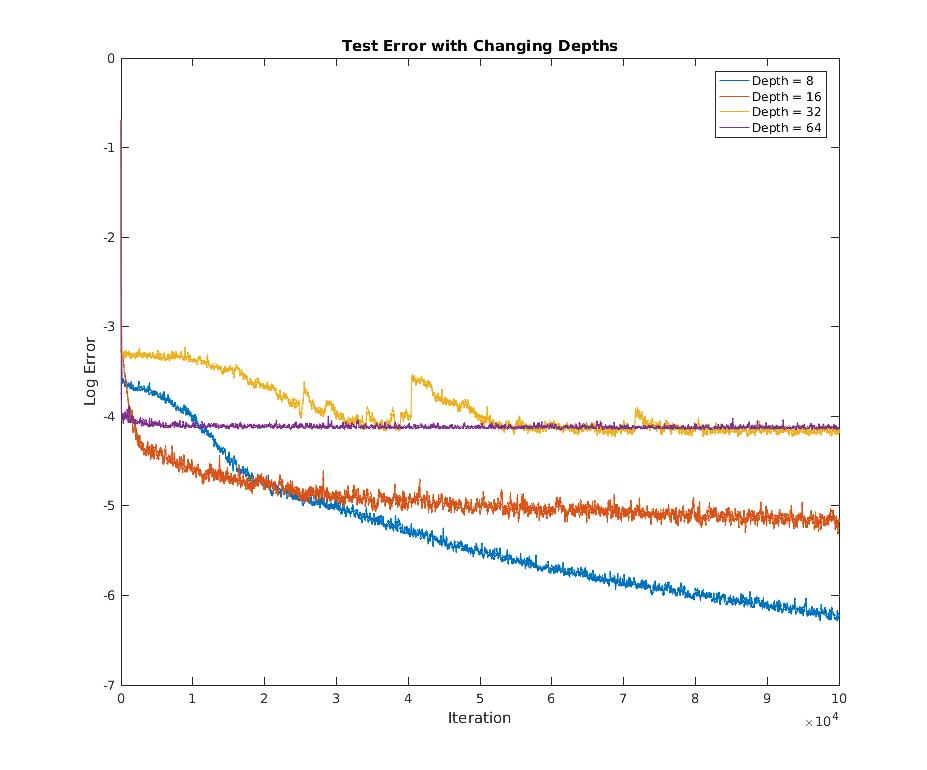
\includegraphics[width = 1.6in]{plotChangeDepth.jpg}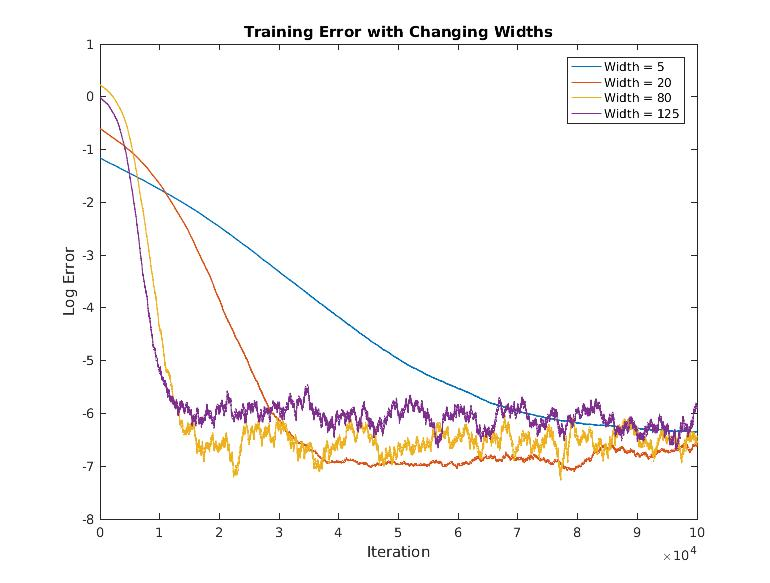
\includegraphics[width = 1.77in]{plotChangeWidth.jpg}
\caption{Left:Test Error of Networks of Varying Depth. Right: Test Error of Networks of Varying Width.}
\end{center}
\vskip -0.1in
\end{figure}
We note that we have been using training error as a measure of success, but it's possible that the true underlying parameters are not learned. If our loss function were strongly convex, small training error would imply a small norm in the parameter space. For the sign activation function, we can show a related result.

\begin{restatable}{theorem}{signUnique}
\label{SignUnique}
Let $\mathcal{M} = S^{d-1}$ and $\sigma$ be the sign activation function and $b_2,...,b_k = 0$. If the loss \eqref{errLoss} at $(a,\theta)$ is less than $O(1)$, then there must exist $\theta_i$ such that $w_1^T\theta_i > \Omega(1/\sqrt{k})$.
\end{restatable}



\section{Conclusion}

In this work, we view deep learning of neural networks in the context of electron-proton dynamics and analyzed the convergence of the underlying weight parameters of the neural network using arguments inspired from physics and non-convex optimization. To do so, we first established mathematical relationship between activation functions and their corresponding potentials. Next, we interpreted gradient descent as electrodynamics under a certain potential. Finally, we discovered classes of activation functions that give rise to positive convergence results, some of which relate to very commonplace activations, such as the sign and polynomial. For these classes of depth-2 neural networks, our results imply that they are provably learnable by deep learning. Our experiments seem to imply that higher depth neural networks are not learnable. 

However, we believe that convergence results for depth-2 neural networks can be extended to even more activation functions, such as the sigmoid or the ReLU. Also, we believe these convergence results can be proven with minimal assumptions. We hope that our work is a step in the theoretical understanding of the performance of neural networks seen in practice.




\bibliographystyle{icml2017}
\bibliography{biblio}

\end{document} 


% This document was modified from the file originally made available by
% Pat Langley and Andrea Danyluk for ICML-2K. This version was
% created by Lise Getoor and Tobias Scheffer, it was slightly modified  
% from the 2010 version by Thorsten Joachims & Johannes Fuernkranz, 
% slightly modified from the 2009 version by Kiri Wagstaff and 
% Sam Roweis's 2008 version, which is slightly modified from 
% Prasad Tadepalli's 2007 version which is a lightly 
% changed version of the previous year's version by Andrew Moore, 
% which was in turn edited from those of Kristian Kersting and 
% Codrina Lauth. Alex Smola contributed to the algorithmic style files.  
